\section{EXPERIMENTS}
\subsection{Experimental Condition}
In this section, we utilize a transformable quad-rotor with four-links. The whole weight is about 3.3[kg]. The three-dimensional position was tracked by a motion capture system, representing nearly ground truth, and sent to the onboard computer via Wi-Fi. The hardware and software system is the same as that explained in Sec. V. The number of target objects was set to 2. Then, using the form optimization method, we calculated optimal forms shown in \figref{quad_state}. The additional mass is 0.551[kg], the sum weight of the target object and the electromagnet gripper. The final values of $V(\bm{u})$ shown under each form, especially that of form (b), are large relatively. The cause is considered that the four-links lacks the degree of freedom of transform due to the contraints described in Sec. IV(b). 
%However, as the forms were optimal, in other words, there can not be more suitable forms, we used the forms.
\begin{figure}[t]
  \begin{center}
    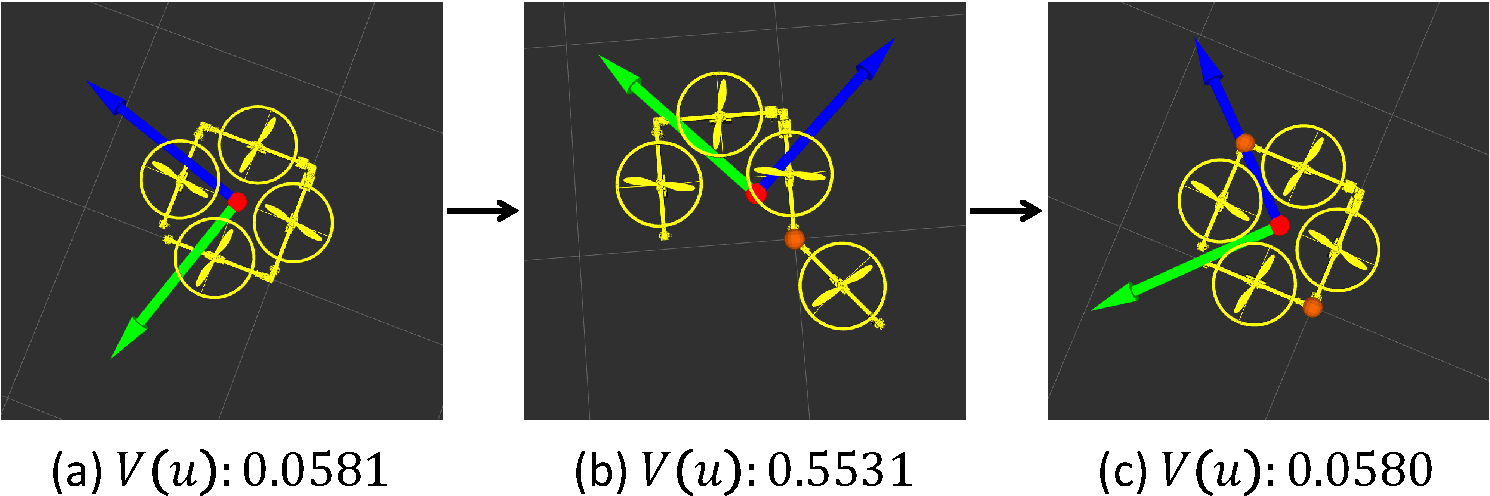
\includegraphics[width=1.0\columnwidth]{figs/quad_state.pdf}
  \end{center}
  \caption{The optimal forms of quad-rotor with four-links: the aerial robot grasps (a):no object (b): one object (c): two objects\label{figure:quad_state}}
\end{figure}

\subsection{Multiple Objects Transportation}
Then, we performed the experiment of multiple object transportation as shown in \figref{experiment}. The process of multiple object transportation can be summarized as follows:$\textcircled{\scriptsize 1}\sim \textcircled{\scriptsize 2}$: approaching to the first object; $\textcircled{\scriptsize 3}\sim \textcircled{\scriptsize 5}$: grasping the first object and transforming to the optimal form(\figref{quad_state}(b)); $\textcircled{\scriptsize 6}\sim \textcircled{\scriptsize 7}$: approaching to the second object; $\textcircled{\scriptsize 8}\sim \textcircled{\scriptsize 10}$: grasping the second object and transforming to the optimal form(\figref{quad_state}(c)); $\textcircled{\scriptsize 11}\sim \textcircled{\scriptsize 12}$: approaching to and landing on the goal aera. The surface of the objects was iron to be able to grasp by the electromagnet gripper. The positions of the objects were tracked by the motion capture system. Note that the optimal forms were calculated in off-line in this work since the weight of the objects were given in advance.
\begin{figure}[t]
  \begin{center}
    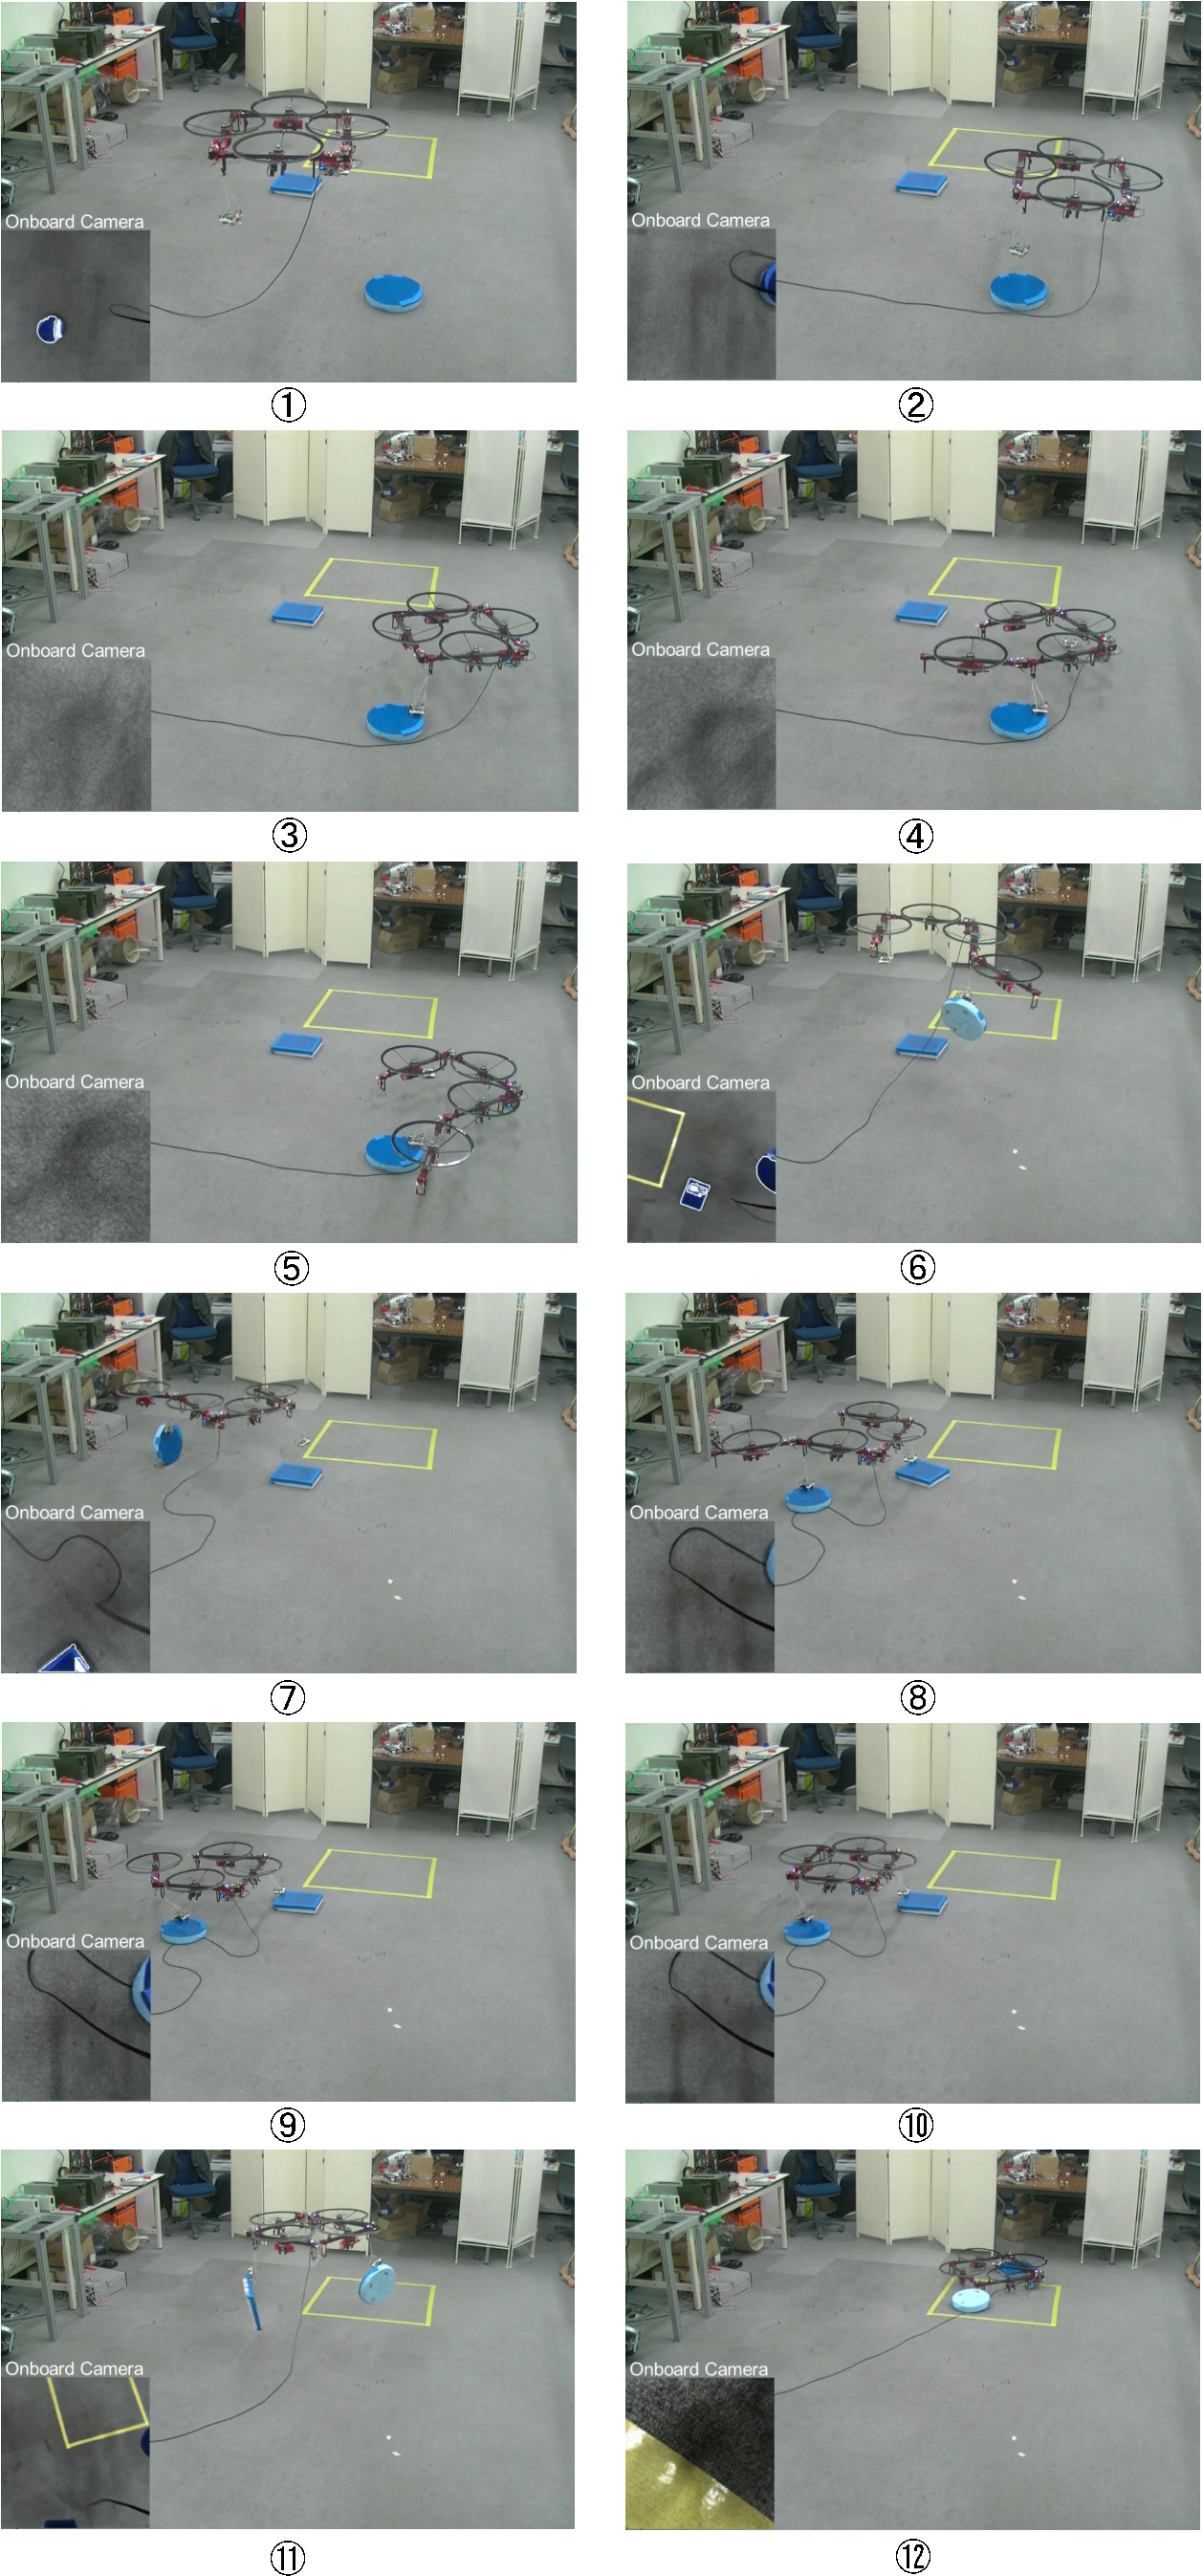
\includegraphics[width=1.0\columnwidth]{figs/experiment.pdf}
  \end{center}
  \caption{Experiment in which two ferrous objects are grasped and transported by the transformable aerial robot.\label{figure:experiment}}
\end{figure}

